\chapter{Workhorse experiment}

In this section, we present the consolidation of our previous experiments in the form of a bigger experiment with a more in-depth analysis.

\section{Repeating elements problem}
\label{SECTION:STACK_STRUCTURE}

Contrary to our intitial expectations, BFPRT parameters did not influence the result when dealing with a sequence with repeated elements. So, for this experiment we change tune a different level, as we now see the structures involved on its resolution.

Reminiscing the main concept of incremental sorting, this approach was designed to tackle the problem of extracting elements from a sequence in a sorted fashion in optimal time when there is no information beforehand on how many elements are needed to be extracted from its source.

In all our previous experiments we always took as granted the definition of our input sequence, which from now we dennote as $S_{in}$. First, $S_{in}$ for all our implementation and structural concerns has a defined size $\norm{S_{in}}$ over a $\mathcal{Z}^{\geq0}$ domain.\footnote{This may seem obvious, but as this structured can be implemented in an arbitrative way, we need to constrain our restrictions for the program as much as possible in order to clearly define our algorithm bounds.} 

Depending on the problem to be solved using IQS/IIQS, we may need different representations for the output. In this regard, we can see IQS and IIQS as a function which maps a sequence $S_{in}$ into another sequence $S_{out}$ which contains the same elements but arranged via a certain criteria. We do not specify the criteria at this point, as it is not the point of this work to compare different comparison mechanisms. For such effects is safe to assume that our comparison criteria is the one in Section~\ref{SEC:INCREMENTAL_SORTING}.

\subsection{Current paradigm}
In rough terms, both IQS and IIQS algorithms belong to the divide-and-conquer paradigm as they recursively break our problem into a smaller ones which are solved later. Contrary to a complete sorting algorithm, on partial sorting we do not expect to solve the problem for our entire input, in other words, we do not need to solve all the recursion steps in the execution tree in order to get an accepted output. 

As a example of this let us consider a sequence $T={4,1,2,3}$. Now let us say that we need a partial sorting over the first two elements of $T$. Then our solutions are $T_1={1,2,3,4}$ and $T_2={1,2,4,3}$. Both $T_1$ and $T_2$ are accepted inputs as the first two elements are sorted. This aforementioned definition does not bound our final implementation to solve all the recursion tree induced by our paradigm and considers this solution as a state of our recursion tree. 

Another ---less graphical--- way of depicting this situation is by modeling our execution tree as a non-deterministic stacked state machine, on which our root node the final node, the leaves of the recursion tree are the initial states (the elements that can be placed in their correct position) with strategically placed elements to be consumed in the stack. There is no need to go through all the states as long as we reach an accepted final state.


In practice\footnote{As another way to say, in common implementations.}, few sorting algorithms run pre-checks in order to avoid certain cases. As these \emph{sanity checks} are bound to cost at least $O(n)$ time, they are not feasible in most cases. That is why introspective algorithms like introsort~\cite{10.5555/261387.261395} and IIQS~\cite{7416566} integrate such process to be part of already existing processes, in order to not affect the overall complexity. 

\subsection{Paradigm shift}
Sequences with repeating elements are a different story. Let us take as example a sequence of elements $T'={1,1,1,1}$, which shares the same size as our previously introduced $T$ sequence, but this one has only one class of elements. Extrapolating the definition of a sequence with only one class among all sequence elements stated in~\ref{SECTION:NOTE_ON_MEDIAN_SELECTION}, this sequence is already sorted as it is. As all the possible permutations on $T'$ share the same values, and the comparison are being made on the values itself, then there is no problem to solve. As our minimal problem has the same size of our original one, our paradigm is no longer valid anymore.\footnote{In fact, the invalidation of the problem paradigm is the real reason behind IIQS failure.}

If we want to continue using IQS or IIQS to solve our incremental sorting problem we first need to validate our paradigm and then solve the problem at hand. Paraphrasing this statement, we need to integrate a process which allows us to map our input to an accepted one without affecting our current complexity.

\subsection{Counting elements to reduce complexity}
As shown in Section~\ref{SUBSECTION:BASE_BENCHMARK}, our ideal input for both IQS and IIQS is a sequence with unique elements. Counting sort already solves this problem by mapping our elements present in $S_{in}$ as a set $C$ of ordered pairs $(v,f)$ on which $v$ is the value in $S_in$, and $v$ is the frequency of the value in $S_in$.~\cite{10.5555/280635} Sorting is achieved by the container of the set or by extending the set to a sequence of elements and storing them accordingly --- this being the preferred way of implementation. 

Unfortunately, while counting sort performs in lineal time, this algorithm does not exhibit a reasonable space-complexity performance when compared to IIQS, as in worst case it requires extra $O(n)$ space whereas IIQS requires $O(log_2(n))$.

\subsection{Mapping}
\label{SECTION:MAPPING}
As shown in Section~\ref{SECTION:NOTE_ON_MEDIAN_SELECTION}, our sorting problem does not take into account the position of the elements and only relies on the value of such elements. This allows us to use the mapping induced by counting sort, $C_{in}$, as a intermediate representation of our original sequence $S_{in}$.

Let us define $S_{repeated(\gamma)}$ as a sequence of elements $(s_0, s_1,...,s_{n-1},s_{n})$ on which $\forall ~s_i \in [0,n]:~s_i = \gamma$. Then every sequence $S_in$ can be seen as a concatenation of $m$ sequences of size $k$ on which $k \leq m$. Then we can establish two functions $roll$ and $unroll$ defined as follows:

\begin{align*}
    roll \colon S_{repeated(\gamma)} &\to C_{\gamma}\\
    (s_0, s_1,...,s_{n-1},s_{n})  &\mapsto (n).
\end{align*}

And analogously:

\begin{align*}
    unroll \colon C_{\gamma} &\to S_{repeated(\gamma)}\\
    (n) &\mapsto (s_0, s_1,...,s_{n-1},s_{n}).
\end{align*}

This mapping allows us to represent any sequence of elements as a sequence of pairs which represent the element and how many repetitions of this element are concatenated to it.\footnote{This representation is also known as \emph{frequency table}.}

\subsection{Integrating counting strategies as a external process}
As both $roll$ and $unroll$ functions operate per each element and not at sequence level we can extend their usage both inside of our current IQS and IIQS implementation or as a external process.

We denote our candidate sorting algorithm as an anonymous function $\lambda_{sort}$. Then our external reduction strategy is as follows:


\begin{algorithm}
\caption{External reduction}\label{ALG:EXTERNAL_IQS}
\begin{algorithmic}[1]
    \Procedure{$external\_strategy$}{$S_{in}, k, \lambda_{sort}$}
    \State $C_{in} \gets roll(S_{in})$
    \State $S_{sorted}' \gets \lambda_{sort}(C_{in}, S, k)$
    \State $S_{out}' \gets [~]$
    \For{$s \in S_{sorted}'$}
        \State $S_{out}' \gets S_{out}'~^\frown~unroll(s, C_{in}(s))$
    \EndFor
    \State \Return $S_{out}$
    \EndProcedure
\end{algorithmic}
\end{algorithm}

Algorithm~\ref{ALG:EXTERNAL_IQS} shows an implementation of a external reduction strategy. We asume that roll operation as it is an instance of counting sort it takes $O(n)$ time and line 4 onwards also take $O(n)$. 

As the average running time for IQS and IIQS is $O(n~+~k~log_2(k))$, then the addition of our external strategy to deal with repeating elements introduces a fixed $n + l$ overhead on which $l$ denotes the number of classes present on $S_{in}$. But this overhead does not change the complexity of both algorithms. But this does not prevent IQS from hitting its worst case scenario unless we control how the keys retrieved from $C_{in}$ are retrieved.

Another drawback of this implementation is that since we are using an external strategy to reduce the repeating elements problem, we need $l$ extra space. In worst case, $l~=~\norm{S_{in}}$, which is suboptimal in relation to IQS.

\subsection{Integrating counting strategies as part of the partition process}

When integrating this problem reduction stage directly into the algorithm, then we need to materialize it at implementation level. For such effects the ideal place to install it in on the stack which tracks the information for the next calls. 

In order to accomplish this, we change the structure of the stack used by extending the operations involved on it, allowing to group a range of of elements instead of just a single element. For such effects, the stack store pairs of elements $u = (p_{start}, p_{end})$ on which $p_{start}$ is the first position of the pivot and $p_{end}$ is the frequency on the array. By extension of the concepts shown in Section~\ref{SECTION:MAPPING} and~\ref{SECTION:NOTE_ON_MEDIAN_SELECTION}, we extend the operations $partition$, $top$ and $pop$ to support both $roll$ and $unroll$ definitions as follows:



\begin{algorithm}
    \caption{Ranged Stack top}\label{ALG:STACK_TOP}
    \begin{algorithmic}[1]
        \Procedure{$Stack.rangedTop$}{$S$}
        \State $(p_{start}, p_{end}) \gets S.top()$
        
        \State \Return $p_{start}$
        \EndProcedure
\end{algorithmic}
\end{algorithm}


\begin{algorithm}
    \caption{Ranged Stack pop}\label{ALG:STACK_POP}
    \begin{algorithmic}[1]
        \Procedure{$Stack.rangedTop$}{$S$}
        \State $(p_{start}, p_{end}) \gets S.top()$
        \State $S.pop()$
    
        \If{$p_{start} < p_{end}$}
            \State $S.push((p_{start}+1, p_{end}))$
        \EndIf
        \EndProcedure
\end{algorithmic}
\end{algorithm}

\begin{algorithm}
\caption{Ranged Three-way Partition}\label{ALG:DUTCH_FLAG_PARTITION_RANGED}
\begin{algorithmic}[1]
    \Procedure{$rangedPartition$}{$A, p$}
    \State $k \gets \norm{A}$
    \State $i \gets 0$
    \State $j \gets 0$
    \While{$j < k$}
        \If{$A_j < p$}
            \State $swap(A_i, A_j)$
            \State $i \gets i+1$
            \State $j \gets j+1$
        \ElsIf{$A_j > p$}
            \State $k \gets k-1$
            \State $swap(A_i, A_k)$
        \Else
            \State $j \gets j+1$
        \EndIf
    \EndWhile
    \State \Return $(i,k)$
    \EndProcedure
\end{algorithmic}
\end{algorithm}

\section{Ranged IIQS}
The extensions shown in Algorithms~\ref{ALG:STACK_TOP}, ~\ref{ALG:STACK_POP} fixes the position of the index returned from the middle section as pivot to the left-most element. As proven in Section~\ref{SECTION:IQS_PARAMS} this bias generates an synthetic best-case execution, which is used directly after the partition stage. Those two algorithms integrate both $roll$ and $unroll$ definitions by storing the range of pivots in a map notation.


On the other hand the extensions for Algorithm~\ref{ALG:DUTCH_FLAG_PARTITION_RANGED} are integrated into IIQS almost directly with no major modifications, allowing a transparent use without any extra overhead, as shown in Algorithm~\ref{ALG:RANGED_IIQS}.

\begin{algorithm}
  \begin{algorithmic}[1]
    \caption{Ranged IIQS} \label{ALG:RANGED_IIQS}
    \Procedure{r-iiqs}{$A, S, k$}
    \While{$k < S.rangedTop()$}
        \State $pidx \gets random(k,S.rangedTop()-1)$
        \State $pidx, range \gets partition(A_{k,S.rangedTop()-1}, pidx)$
        \State $m \gets S.rangedTop() - k$
        \State $\alpha \gets 0.3$
        \State $\beta \gets 0.7$
        \State $idx_\alpha \gets k + \alpha m$
        \State $idx_\beta \gets k + \beta m$
        \State $r \gets -1$

        \If{$pidx > idx_\beta \wedge idx_\alpha < pidx $}
            \State $pidx \gets pick(A_{r+1,S.rangedTop()-1})$
            \State $pidx, range \gets rangedPartition(A_{r+1,S.rangedTop()-1},pidx)$
        \EndIf
        \State S.push($(pidx, range)$)

    \EndWhile
    \State S.pop()
    \State \textbf{return} $A_{k}$\label{IIQS_main_cycle}
    \EndProcedure
  \end{algorithmic}
\end{algorithm}

As both Algorithms~\ref{ALG:STACK_TOP}, ~\ref{ALG:STACK_POP} have $O(1)$ worst-case complexity and Algorithm~\ref{ALG:DUTCH_FLAG_PARTITION_RANGED} maintains $O(n)$ complexity on which $n$ dennotes the number of elements in the sequence to partition. Both expected and worst-case time complexity for this \emph{Ranged IntrospectiveIncrementalQuickSort} (\emph{rIIQS} from now on) remains $O(n~+~k~log_2(k))$ and our original $O(log_2(k))$ space complexity is maintained as the stack only doubles its size at most.

As elements in the stack are stored as a pair, this enables the use or custom structures to store such pairs, which enables a better use of DRAM bursts on the target machine. This guarantees a nearly zero overhead on read and write operations for the stack.

The experiments developed on Sections~\ref{SECTION:IQS_PARAMS} also helps us to fix our parameters for the execution of the introspective steps to $\alpha=0.5$ and $\beta=0.65$ as experimentally has been proven to offer the best performance from all tested combinations.

This makes \emph{rIIQS} a direct replacement of \emph{IIQS} for all cases. Additionally, if worst-case execution is not relevant, the same modifications are available for its use on \emph{IQS} implementations in order to support repeated elements on its input.

\section{Experimental evaluation}

Now we present the experimental results for our proposed implementation of rIIQS against our existing implementations of IQS and IIQS to validate our aforementioned proposals.


\subsection{Performance comparison for unique sequences}

Experments have shown that rIIQS does not induce an increase of the algorithm complexity for our standard test cases such as random sequences, ascending sorted sequences and descending sorted sequences, as shown in detail in Figures~\ref{FIG:WORKHORSE_BENCHMARK_01},~\ref{FIG:WORKHORSE_BENCHMARK_02} and ~\ref{FIG:WORKHORSE_BENCHMARK_03}. For then, our hypothesis on the equivalence of IIQS and rIIQS for our base IQS test cases is confirmed. 

\begin{figure}[!ht]
    \centering
    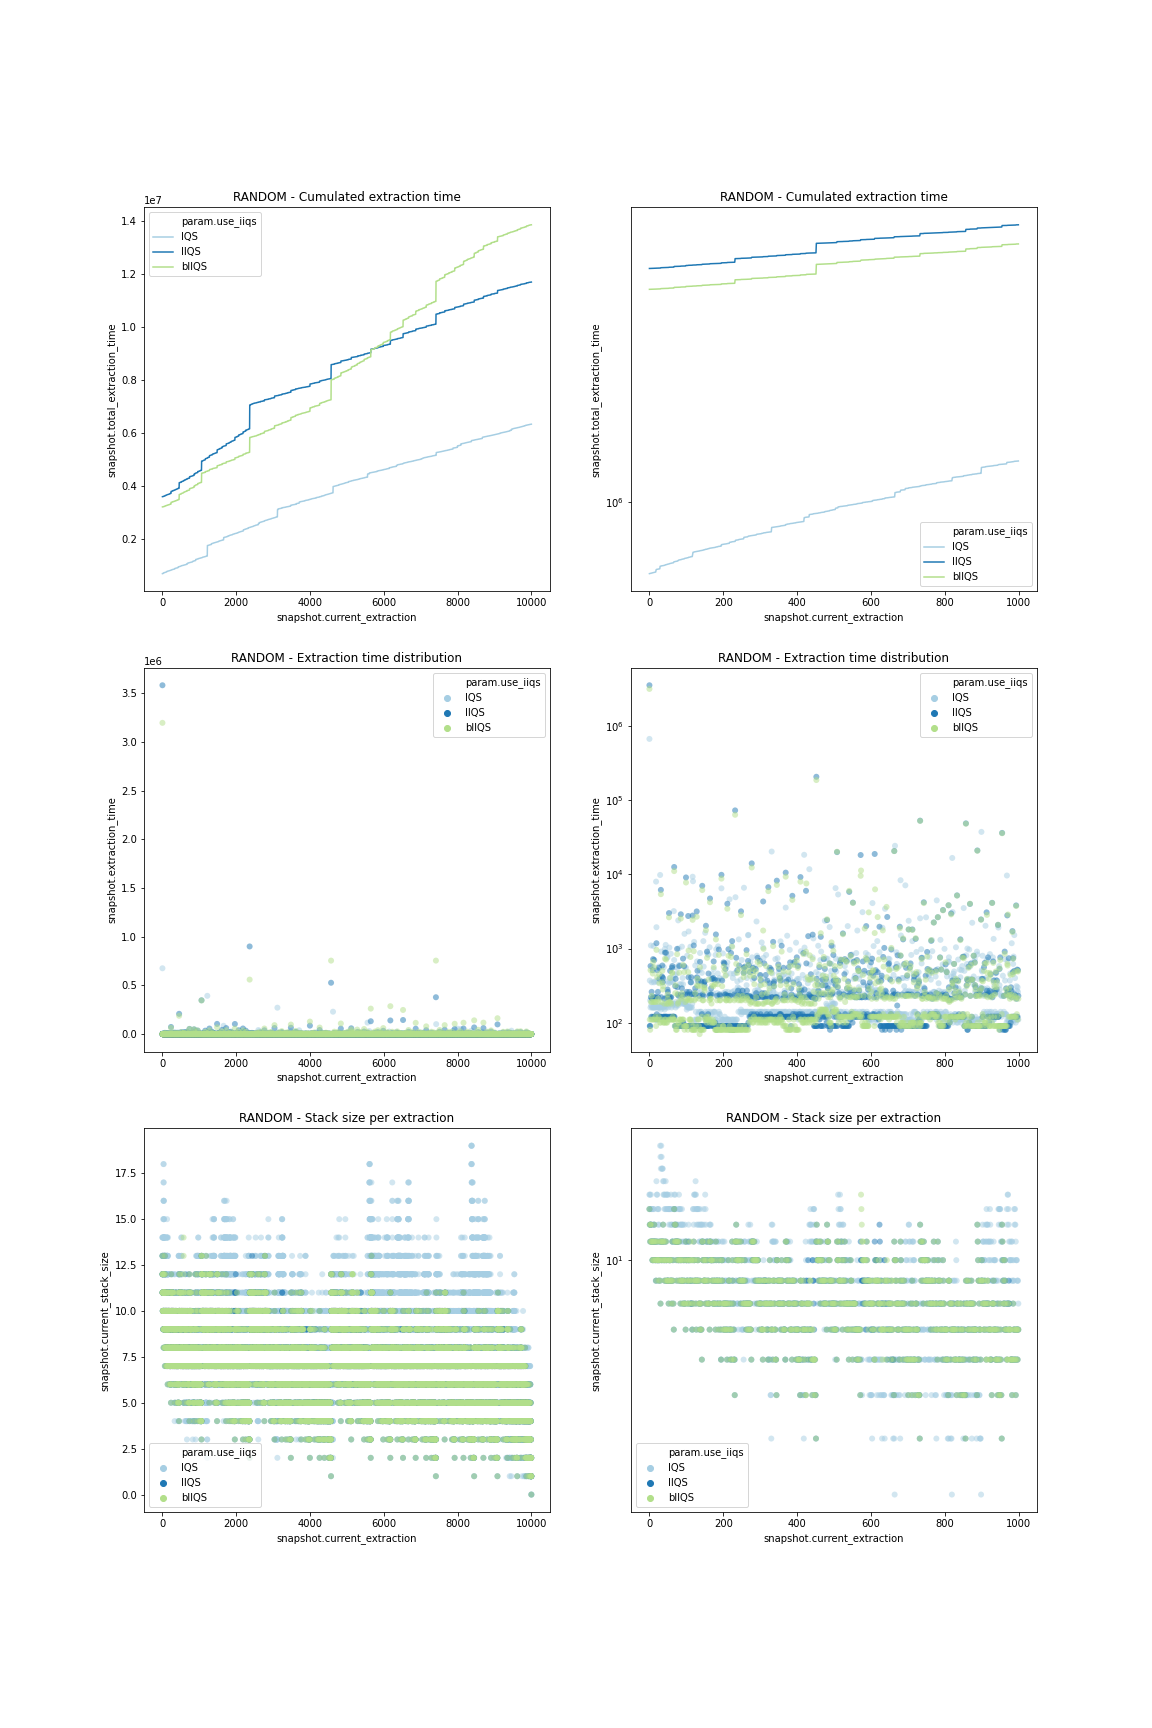
\includegraphics[width=0.8\textwidth]{./fragments/05_workhorse_experiment/images/01_basebenchmark_01_random_case.png}
    %\caption{Benchmark for random case. IQS and IIQS executions are shown on the first and second columns respectively.}
    \caption{Benchmark for rIIQS using elements $1\times10^4$ as a randomly sorted sequence. IQS and IIQS executions are shown on the first and second column respectively. All extractions using a symlog scale.}
    \label{FIG:WORKHORSE_BENCHMARK_01}
\end{figure}

\begin{figure}[!ht]
    \centering
    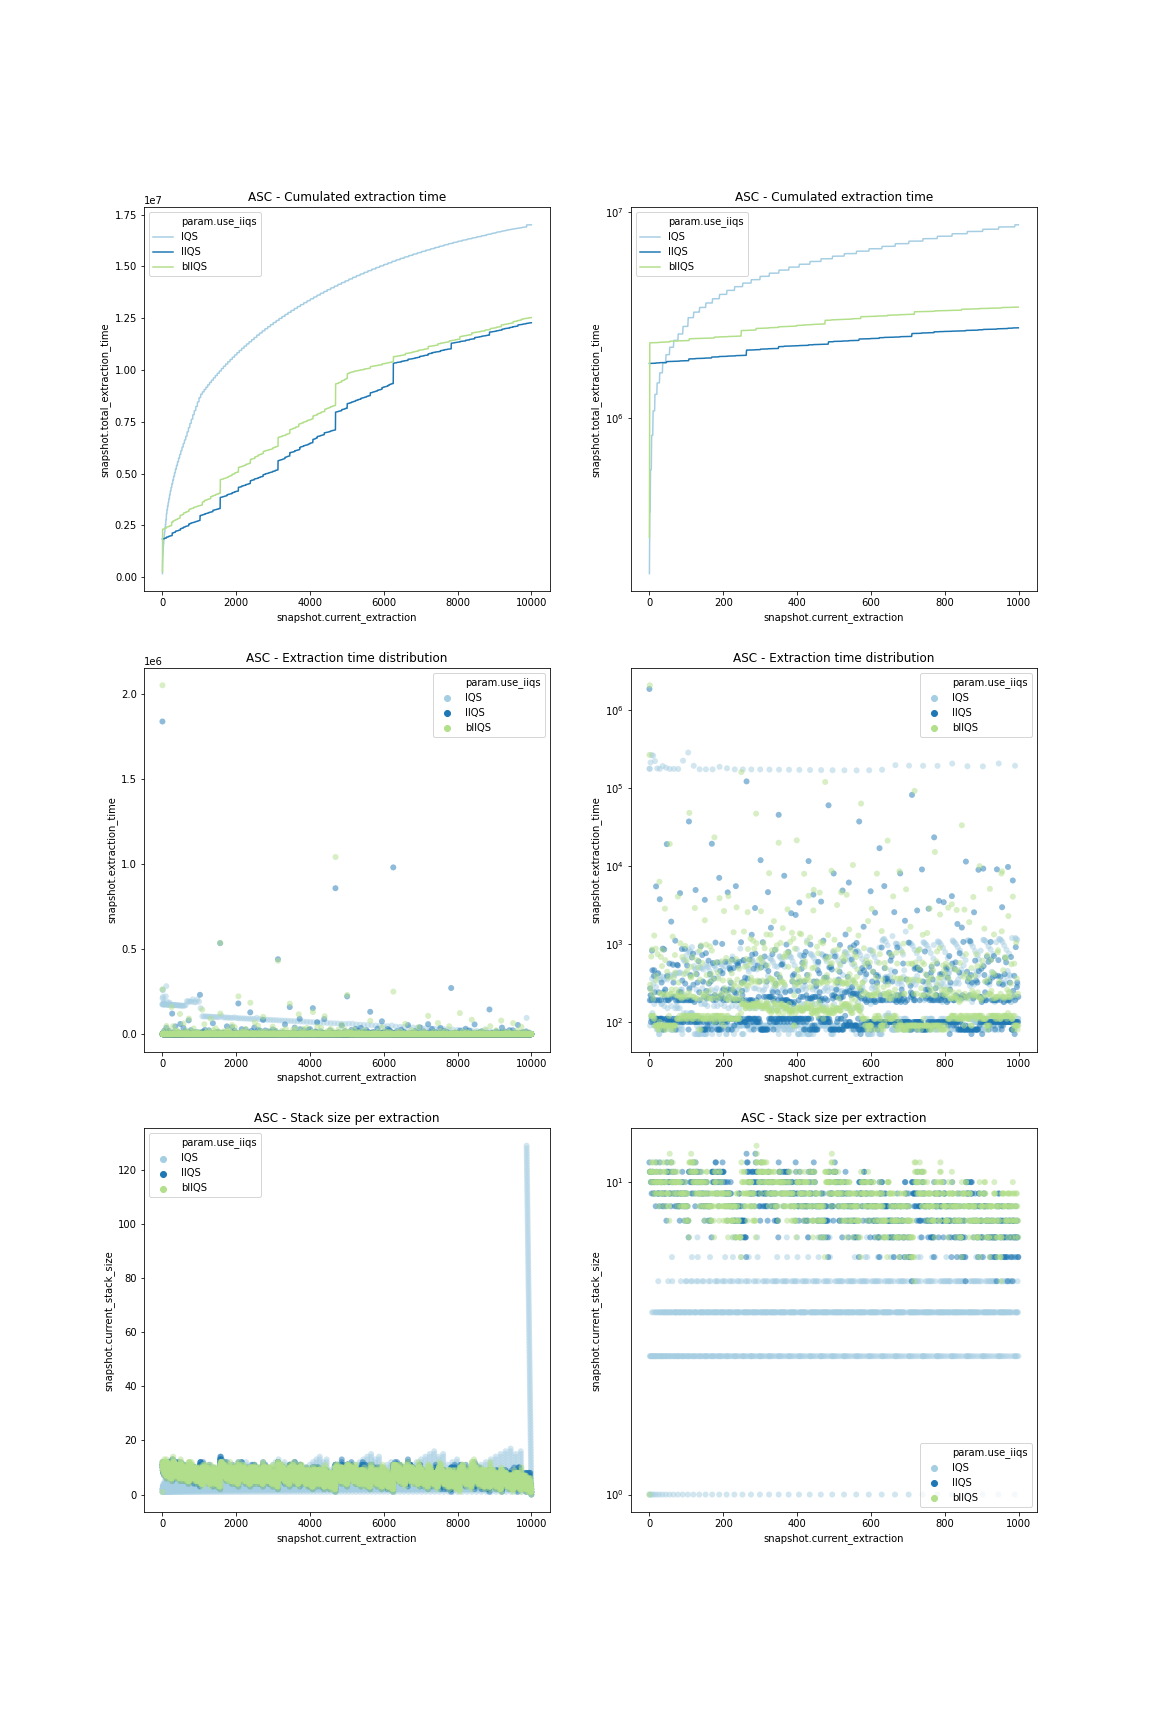
\includegraphics[width=0.8\textwidth]{./fragments/05_workhorse_experiment/images/01_basebenchmark_02_sort_a_case.png}
    %\caption{Benchmark for random case. IQS and IIQS executions are shown on the first and second columns respectively.}
    \caption{Benchmark for rIIQS using elements $1\times10^4$ as a ascending sorted sequence. IQS and IIQS executions are shown on the first and second column respectively. All extractions using a symlog scale.}
    \label{FIG:WORKHORSE_BENCHMARK_02}
\end{figure}

\begin{figure}[!ht]
    \centering
    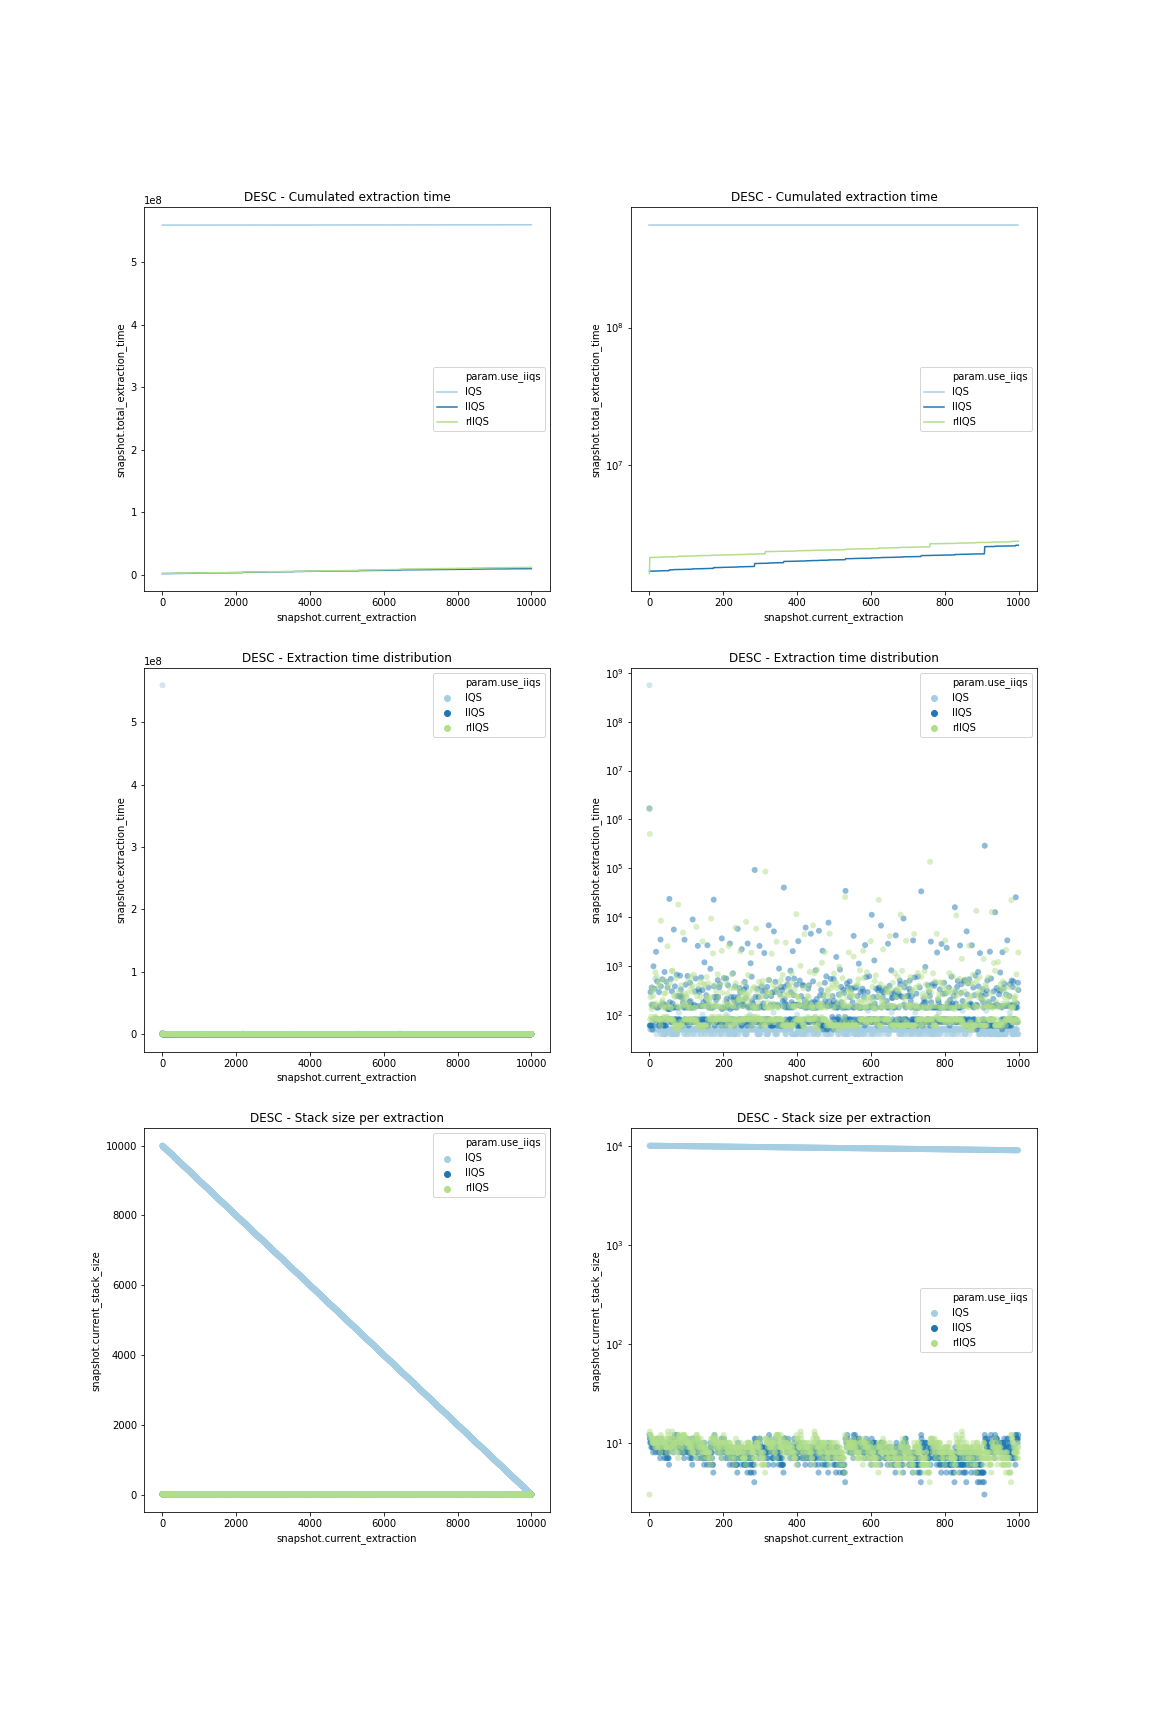
\includegraphics[width=0.8\textwidth]{./fragments/05_workhorse_experiment/images/01_basebenchmark_03_sort_d_case.png}
    %\caption{Benchmark for random case. IQS and IIQS executions are shown on the first and second columns respectively.}
    \caption{Benchmark for rIIQS using elements $1\times10^4$ as a descending sorted sequence. IQS and IIQS executions are shown on the first and second column respectively. All extractions using a symlog scale.}
    \label{FIG:WORKHORSE_BENCHMARK_03}
\end{figure}

\FloatBarrier
\subsection{Performance comparison for repeated sequences}

For single class instances which represent the worst case for IIQS when dealing with repeated sequences, rIIQS shows more than three orders of magnitude boost in performance in comparison to IIQS. As shown in Figure~\ref{FIG:WORKHORSE_BENCHMARK_05}, while our single class input continues to represent our worst case, it does not pose a problem as before. Experimental results shown in Figure~\ref{FIG:WORKHORSE_BENCHMARK_04} reveal that rIIQS does not only perform a fastest first element extraction, but also that formerly stated properties of IIQS as optimal space usage and fastest extractions are also preserved. As the stack now stores a range of elements, each extraction performed on it does not require any extra partition stage as it is being immediately delivered. This makes the ---optional--- pop-push operation the only overhead in this implementation.

\begin{figure}[p]
    \centering
    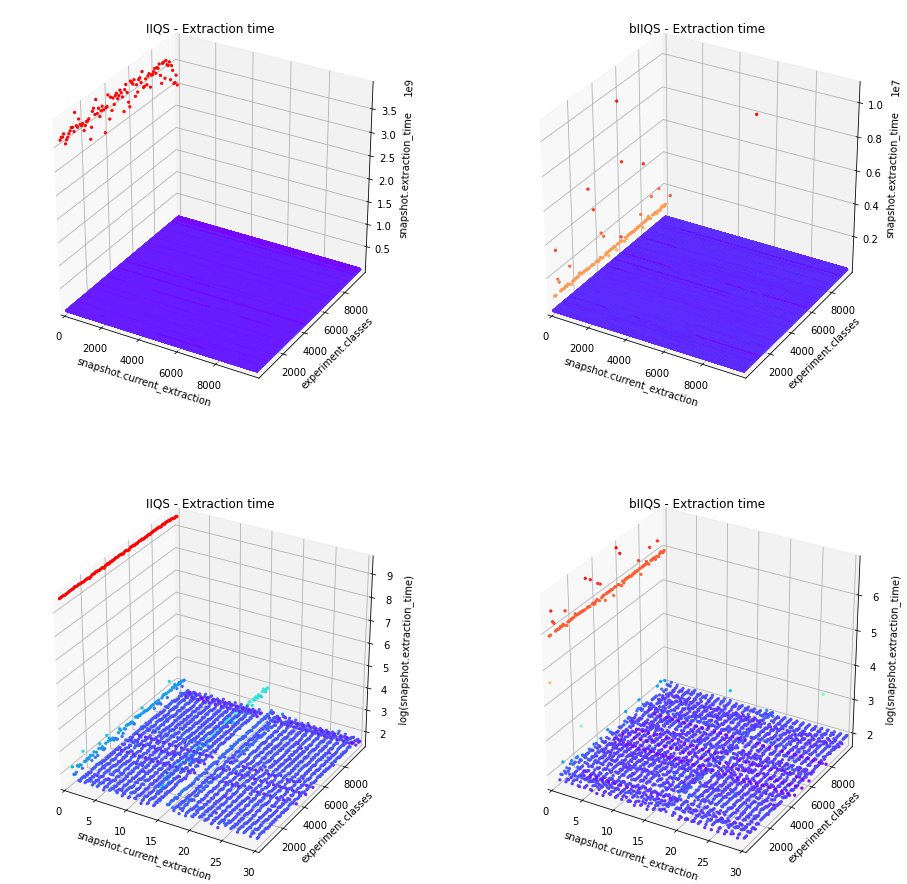
\includegraphics[width=0.8\textwidth]{./fragments/05_workhorse_experiment/images/01_basebenchmark_05_classes.png}
    %\caption{Benchmark for random case. IQS and IIQS executions are shown on the first and second columns respectively.}
    \caption{Benchmark for rIIQS using $1\times10^4$ elements for sequences with a variable number of classes. IQS and IIQS executions are shown on the first and second column respectively. All extractions using linear symlog scale.}
    \label{FIG:WORKHORSE_BENCHMARK_05}
\end{figure}


\begin{figure}[p]
    \centering
    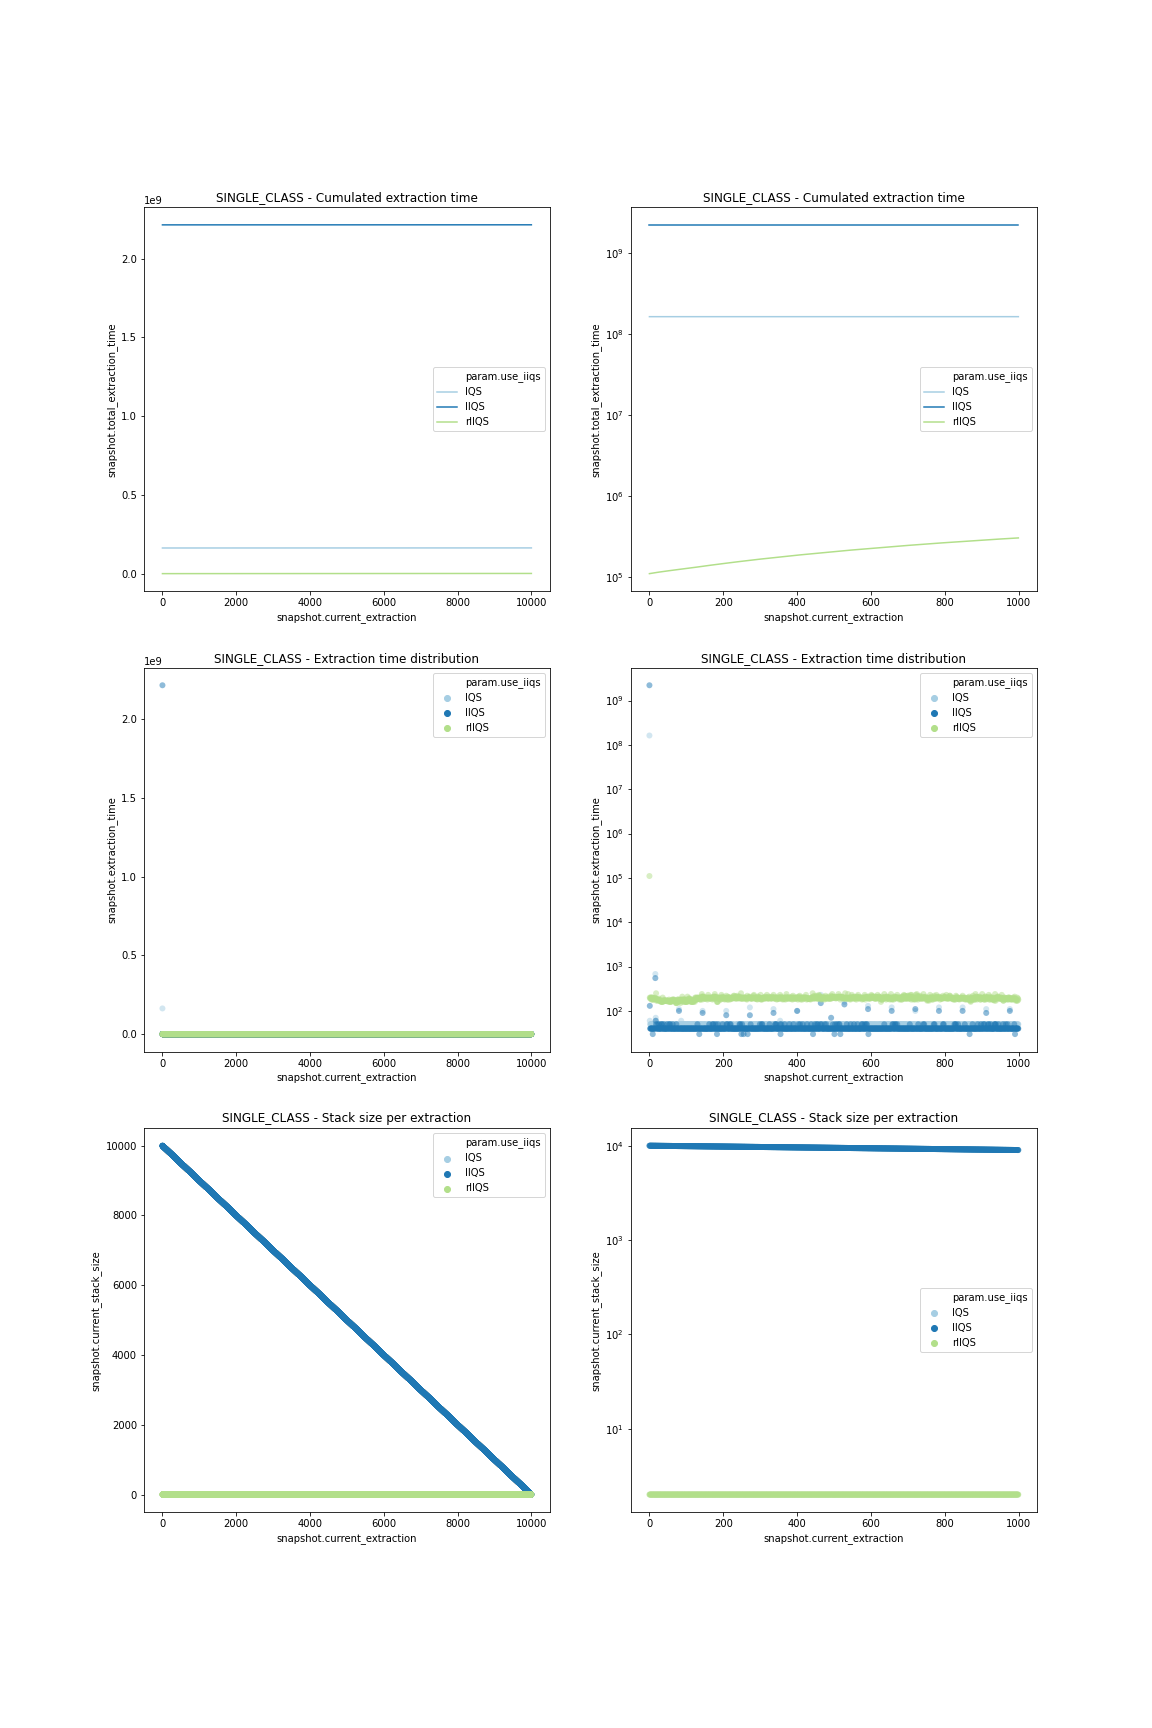
\includegraphics[width=0.8\textwidth]{./fragments/05_workhorse_experiment/images/01_basebenchmark_04_single_class.png}
    %\caption{Benchmark for random case. IQS and IIQS executions are shown on the first and second columns respectively.}
    \caption{Benchmark for rIIQS using $1\times10^4$ elements for sequences with a single class spanned on it. IQS and IIQS executions are shown on the first and second column respectively. All extractions using linear symlog scale.}
    \label{FIG:WORKHORSE_BENCHMARK_04}
\end{figure}


As for the noise impact we can clearly identify that now the bias on the resulting index provided by the three-way partition does not impact on the performance of rIIQS except for very small values (see Figure~\ref{FIG:WORKHORSE_BENCHMARK_05}). In contrast, the noise now has a slight negative impact on rIIQS which can be attributed to the extra step performed to stack a pair of elements instead of a single one. Even with this degradation, the performance on all cases is stable in comparison to IIQS and delivers results in the expected running time, on par with random sequences of unique elements.

\begin{figure}[!ht]
    \centering
    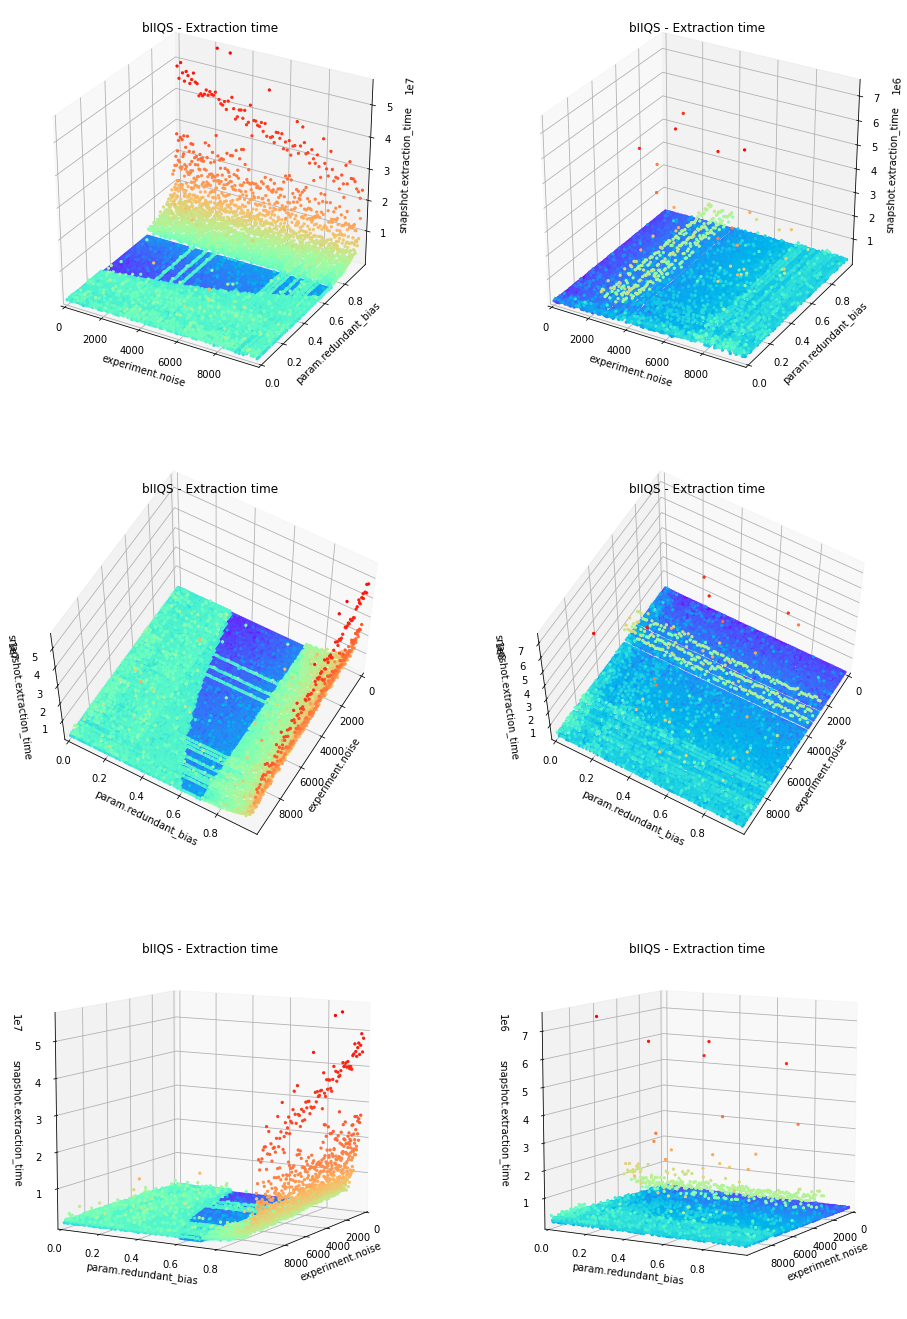
\includegraphics[width=0.8\textwidth]{./fragments/05_workhorse_experiment/images/01_basebenchmark_06_noise_redundant_bias.png}
    %\caption{Benchmark for random case. IQS and IIQS executions are shown on the first and second columns respectively.}
    \caption{Benchmark for rIIQS using $1\times10^4$ elements for sequences with a single class spanned on it with variable noise and three-way-partition bias. IQS and IIQS executions are shown on the first and second column respectively. Only first extraction is shown.}
    \label{FIG:WORKHORSE_BENCHMARK_05}
\end{figure}

We confirm our hypothesis by examining both noise impact and three-way-partition bias as separate elements depicted in Figures~\ref{FIG:WORKHORSE_BENCHMARK_06} and Figures~\ref{FIG:WORKHORSE_BENCHMARK_07} respectively.

\begin{figure}[!ht]
    \centering
    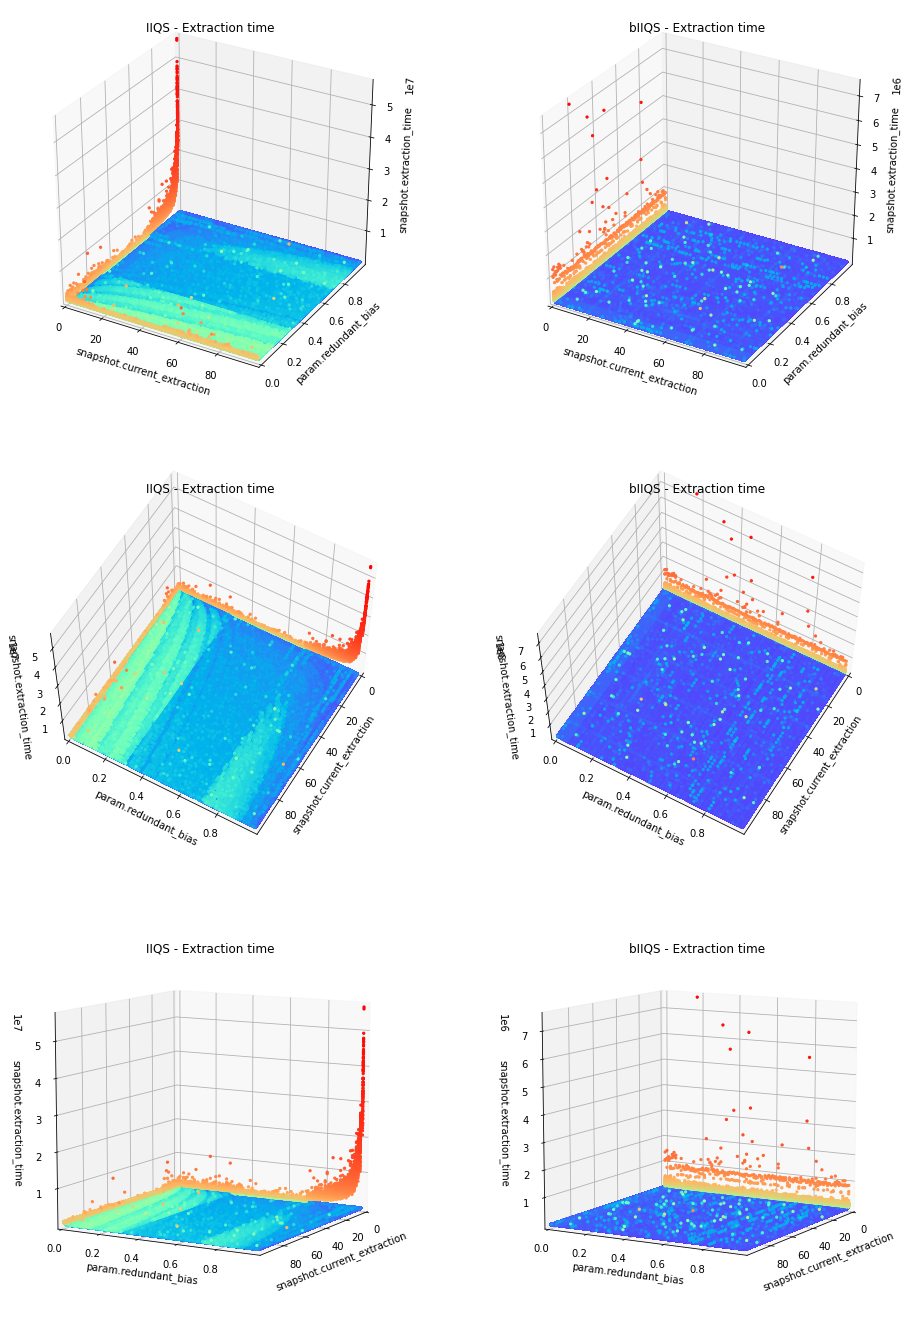
\includegraphics[width=0.8\textwidth]{./fragments/05_workhorse_experiment/images/01_basebenchmark_06_redundant_bias.png}
    %\caption{Benchmark for random case. IQS and IIQS executions are shown on the first and second columns respectively.}
    \caption{Benchmark for rIIQS using $1\times10^4$ elements for sequences with a single class spanned on it with variable noise and three-way-partition bias. IQS and IIQS executions are shown on the first and second column respectively. All extractions using a linear scale.}
    \label{FIG:WORKHORSE_BENCHMARK_06}
\end{figure}

\begin{figure}[!ht]
    \centering
    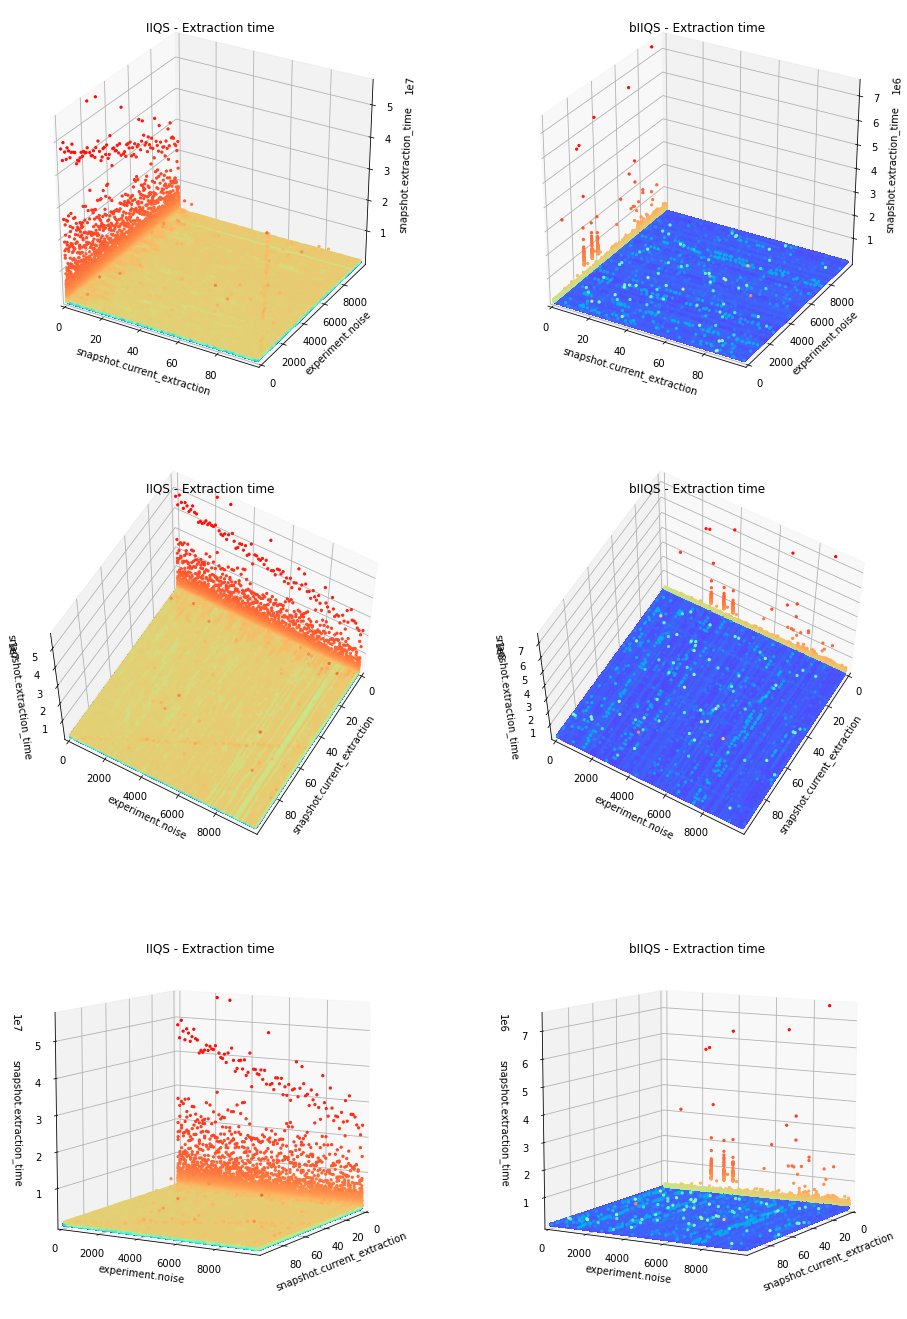
\includegraphics[width=0.8\textwidth]{./fragments/05_workhorse_experiment/images/01_basebenchmark_06_noise_bias.png}
    %\caption{Benchmark for random case. IQS and IIQS executions are shown on the first and second columns respectively.}
    \caption{Benchmark for rIIQS using $1\times10^4$ elements for sequences with a single class spanned on it with variable noise and three-way-partition bias. IQS and IIQS executions are shown on the first and second column respectively. All extractions using a linear scale.}
    \label{FIG:WORKHORSE_BENCHMARK_07}
\end{figure}
